% !TeX root = ../tesis.tex

\chapter{Teoría}
\label{chapter:theory}

\vspace*{7em}

It is recommended to write a summary about the contents of this chapter as an introduction to them. 

\blindtext

\section{Esparcimiento de ondas electromagnéticas}
\label{section:basics}

If you want to frame some equations because you consider them important, use the \textbf{tcolorbox} command. Also, you may use the \textbf{subequations} command sometimes. Fot example with the Maxwell's equations \cite{griffiths2013electrodynamics}:\vspace*{-.75em}
%
	\begin{subequations} \label{eqs:Maxwell}
	\begin{tcolorbox}[title = Ecuaciones de Maxwell en el sistema internacional de unidades,
	ams align, breakable]
	\nabla \cdot\vb{E} &= \frac{\rho_{tot}}{\varepsilon_0}, &\mbox{(Ley de Gauss eléctrica)}  
	\label{seq:GE} \\
	\nabla \cdot\vb{B} &= 0,						&\mbox{(Ley de Gauss magnética)}   
	\label{seq:GM} \\
	\nabla \times\vb{E} &= -\pdv{\vb{B}}{t}, 	&\mbox{(Ley de Faraday-Lenz)}		
	\label{seq:FL}\\
	\nabla \times\vb{B} &= \mu_0 \vb{J}_{tot} +\varepsilon_0\mu_0 \pdv{\vb{E}}{t}, &
	\mbox{(Ley de Ampère-Maxwell)} \label{seq:AM}
	\end{tcolorbox}\end{subequations}\vspace*{-.75em}\noindent
%
and if you want them to appear in the analytical index just use the \textbf{index} command \textbackslash index\{ \}.\index{Maxwell!ecuaciones de}

If you want to show two equations in only one row, use the macros \textbf{\textbackslash eqhalf}, for example\cite{hecht1998optics} \index{Ecuación!de onda}, for the Fourier transform \footnote{\setstretch{1.0} $\mathcal{F}[f(\vb{r},\omega)] = \int_{-\infty}^\infty f(\vb{r},t) e^{i(\vb{k}\cdot\vb{r} -\omega t)} dt$, con $\vb{k}$ una función de $\omega$. La transformada de Fourier inversa es entonces $\mathcal{F}^{-1}[f(\vb{r},t)] =\frac{1}{2\pi} \int_{-\infty}^\infty f(\vb{r},\omega) e^{i(\vb{k}\cdot\vb{r} -\omega t)} d\omega$.\index{Fourier! Transform}} or the Helholtz equation \index{Equation! Helmholtz} for $\vb{E}$ y $\vb{B}$ \cite{griffiths2013electrodynamics}

	\begin{subequations}%
	\eqhalf{\nabla^2\vb{E} + k^2 \vb{E}=\vb{0},}%
	\eqhalf{\nabla^2\vb{B} + k^2 \vb{B}=\vb{0}.}\label{eq:Helmholtz}%
	\end{subequations}\vspace*{-1em}

\noindent leading to plane waves as follow

	\begin{subequations}%
	\eqhalf{\vb{E}(\vb{r},t) =\vb{E_0}e^{i(\vb{k}\cdot\vb{r} -\omega t)},}%
	\eqhalf{\vb{B}(\vb{r}, t) =\vb{B_0}e^{i(\vb{k}\cdot\vb{r} -\omega t),}}	
	\label{eqs:ondasPlanas}\end{subequations}\vspace*{-1em}
		
\noindent \blindtext \vspace*{-.75em}
%
	\begin{tcolorbox}[title = Índice de refracción, ams align]
	n(\omega) = \sqrt{\frac{\mu\varepsilon(\omega)}{\varepsilon_0 \mu_0}}.
		\label{eq:indice} 
	\end{tcolorbox}\vspace*{-.75em}

For the figures, you can use this format:
%
	\begin{figure}[h!]\centering
	\begin{subfigure}{.05\textwidth}%
		\caption{}\label{sfig:secondary1}\vspace*{5cm}
	\end{subfigure}
	\begin{subfigure}{.43\textwidth} 
			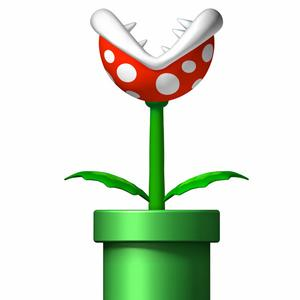
\includegraphics[width=\linewidth]{1-Theory/figs/plant}		
	\end{subfigure}
	\begin{subfigure}{.05\textwidth}%
		\vspace{-5cm}\caption{}\label{sfig:secondaty2}
		\end{subfigure}
	\begin{subfigure}{.43\textwidth} 
			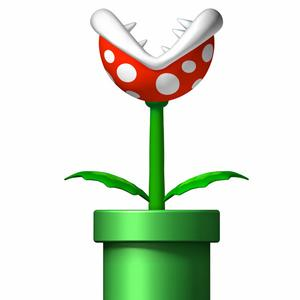
\includegraphics[width=\linewidth]{1-Theory/figs/plant}
	\end{subfigure}%
	\vspace*{-.25cm}
	\caption{The explanation of your figures. \blindtext}	\label{fig:Main}	
	\end{figure}	
				
\Blindtext
